\subsection{Projekt Hydronaut}
\label{subsec:projekt_hydronaut}
Projekt Hydronaut začal jako podvodní komora, která se postupně proměnila v
laboratoř s celým logistickým a vědeckým zařízením. Nyní slouží pro různorodé
výzkumné účely, včetně zkoumání vlivu izolace a extrémního prostředí na psychiku
člověka a testování technologií za extrémního tlaku.

\subsection{Výběr posádky}
\label{subsec:vyber_posadky}
Výběr posádky pro misi DIANA začal s půlročním předstihem v podobě týmové a
individuální diagnostiky posádky. Tato část byla primárně realizována
psychologickým týmem Filozofické fakulty Univerzity Palackého v Olomouci. Byly
využity neuropsychologické, dotazníkové a škálové metody, přičemž také proběhli
motivační rozhovory na téma pobytu v ICE prostředí. Výsledky testů byly zároveň
použity pro ladění všech psychologických nástrojů a aspektů pro samotnou misi
včetně realizace mise samotné.

Při této příležitosti také proběhly i různorodé technické testy. Všechny
výsledky byly důležité primárně pro přípravu detailního programu celé mise tak,
aby co nejdůvěrohodněji simulovala pobyt v ICE prostředí, včetně minutového
harmonogramu zaměřeného na technická, lékařská, psychologická a sociální
hlediska pobytu. Harmonogram je dále popsán v
sekci~\ref{subsubsec:harmonogram_mise}.

\subsection{Posádka pro misi DIANA}
Pro misi DIANA byla vybraná šestice členů posádky. Tři jedinci na plovoucí
platformě (mateřská loď) a další tři pro podvodní stanici (přistávací modul).
Vybraný vzorek se skládal z mužů ve věkovém rozmezí 25--58 let, kteří předem
podstoupili vstupní lékařskou prohlídku. Výběr proběhl na základě preselekce
popsané v předchozí sekci. Žádnému jedinci nebyla diagnostikována žádná
kardiovaskulární onemocnění, ani jiné zdravotní problémy, které by mohly být
stěžejní pro misi. V rámci posádky přistávacího modulu se jednalo o trénované
potápěče vzhledem k saturačnímu pobytu pod hladinou.

\subsection{Popis lokality a podmínky prostředí}
\label{subsec:diana_lokalita}
Stanice H03 DeepLab je lokalizována v lomu Jesenný. Obec Jesenný se nachází v
okrese Semily (Liberecký kraj). Jedná se o zatopený vápencový lom s rozlohou
130x90~\si\meter~a maximální hloubkou 13,5~\si\meter. Vzhledem k tomu, že mise
probíhala pod vodní hladinou, tak nadále nebude uveden geologický kontext
lokality. V průběhu celého experimentu byly příznivé podmínky počasí a
nevyskytly se žádné extrémní události, které by misi ohrožovaly.

\begin{figure}[h]
    \begin{center}
        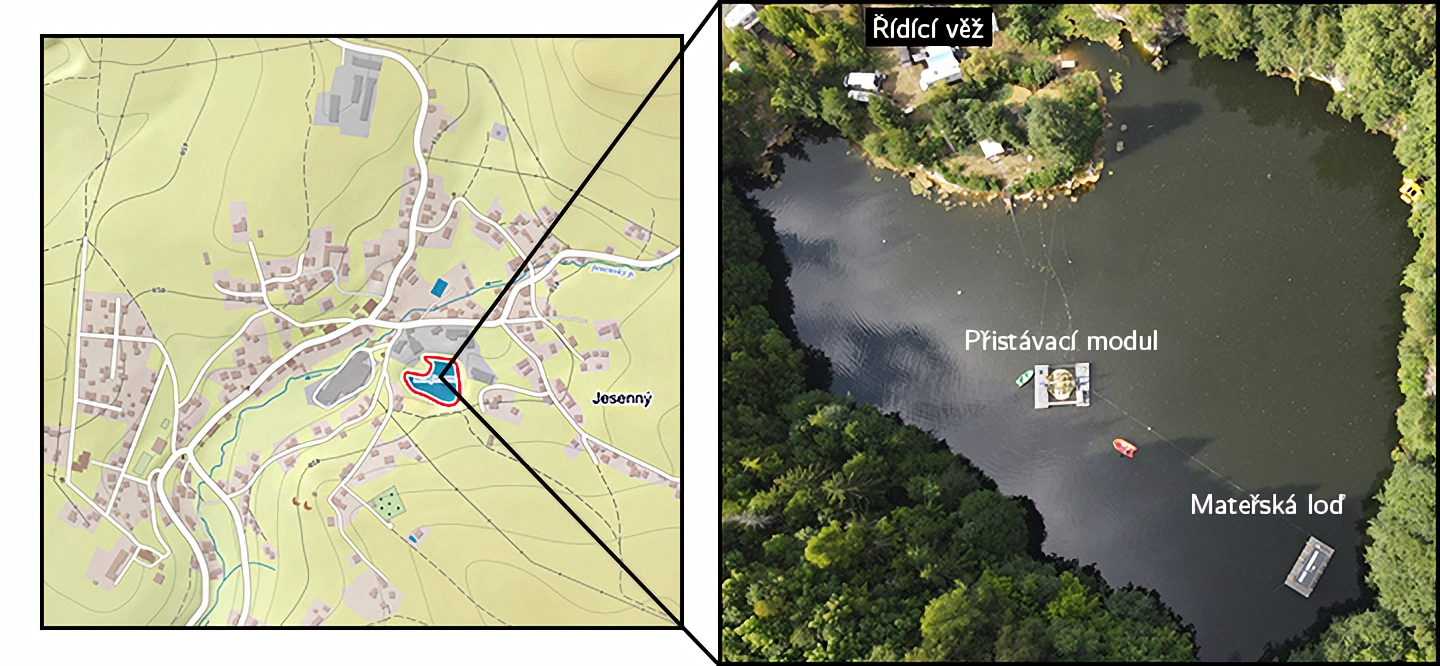
\includegraphics[width=1\linewidth]{figures/map}
        \caption{Detail a lokalita lomu v obci Jesenný (zdroj mapového podkladu: Mapy.cz)}
        \label{fig:map}
    \end{center}
\end{figure}

\subsection{Hlubinná laboratoř H03 DeepLab}
\label{subsubsec:h03_deeplab}
Hydronaut H03 DeepLab je jedinečná výzkumná podvodní laboratoř pro výcvik
posádek v \gls{ICE} podmínkách. Stanice byla zřízena tak, aby umožnila
dlouhodobý pobyt tří členů posádky pod vodní hladinou, přičemž její konstrukce
kombinuje kesonový a ponorkový princip. Díky této unikátní laboratoři bylo tak
umožněno vytvořit podmínky pro dlouhodobý výzkum a sledování vlivu tlaku,
vlhkosti, stresu, umělého osvětlení a izolovaného prostředí na člověka, nebo
použité materiály a vybavení. V rámci mise DIANA plnila stanice roli
přistávacího modulu.

\begin{figure}[h]
    \begin{center}
        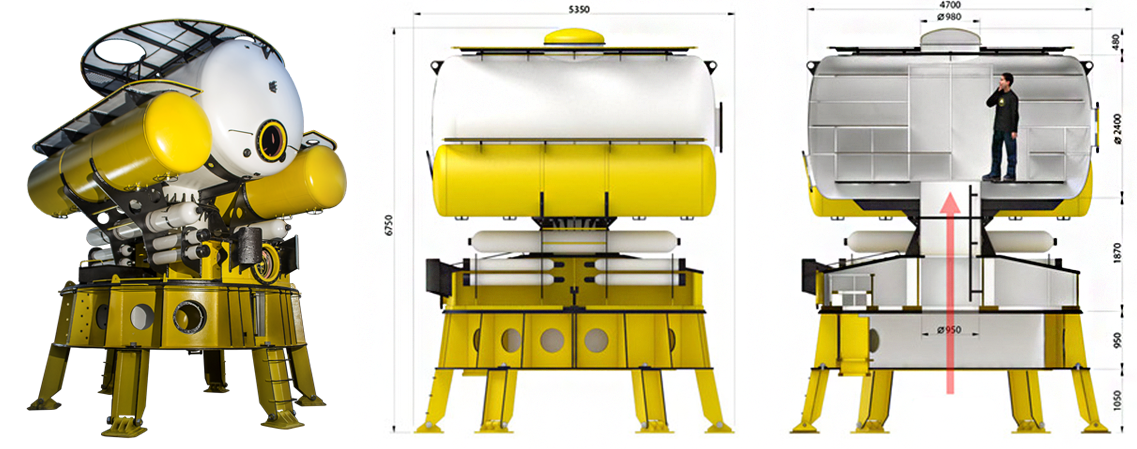
\includegraphics[width=1\linewidth]{figures/habitat}
        \caption{Hlubinná laboratoř H03 DeepLab a její schéma (zdroj: Hydronaut Project a.s.)}
        \label{fig:habitat}
    \end{center}
\end{figure}

\subsubsection{Vybavení stanice}
\label{subsubsec:vybaveni_stanice}
Po hardwarové stránce je stanice je vybavena systémy pro monitorování stavu
prostředí uvnitř habitatu a pro monitorování fyziologických funkcí jednotlivých
členů posádky. Součástí je také systém pro přenos dat do řídícího stanoviště.

Pro potřeby komunikace nebo monitorování fyziologických dat je stanice vybavena
i potřebným softwarem, který je integrován do škálovatelného palubního systému.
Systém umožňuje vizualizaci, administraci a hodnocení měřených enviromentálních
a biomedicínských veličin (data prostředí, biomedicínská data) společně s
obousměrnou komunikaci se všemi zapojenými účastníky s možností volby různých
komunikačních omezení (např. pro potřeby simulace výpadku komunikace). Vybrané
dílčí části vybavení stanice jsou detailněji popsány v následujících sekcích.

\subsubsection{Řízení stanice a mise}
\label{subsubsec:rizeni_stanice_mise}
Stanice H03 DeepLab má hlavní komunikační systém zvaný \textit{Common Tongue}.
Ten zajišťuje komunikaci mezi posádkou a podpůrným týmem a umožňuje živé
sledování životních funkcí posádky a vnitřního prostředí. Pomocí tohoto systému
byly subjektům experimentu zadávány úkoly. Jednotlivé úkoly byly sledovány za
účelem vyhodnocení změn chování vlivem stresu na soustředění a výkonnost mozku.

\subsubsection{Monitorování atmosféry habitatu}
Jedním z důležitých východisek pobytu v habitatu jsou podmínky prostředí, které
je nezbytné nepřetržitě a spolehlivě monitorovat. Jednou z těchto podmínek je
atmosféra pro jejíž monitorování slouží systém založený na platformě slowRIO
(slow remote IO controller) vyvinutý Fakultou strojní (FS ČVUT) na projektu
Hydronaut. Systém monitoruje a poskytuje data prostředí -- mikroklima: absolutní
tlak, relativní vlhkost, teplota vzduchu a vody, čidlo $O_2$, čidlo $CO_2$,
čidlo $H_2$, čidlo $CH_4$, intenzita osvětlení, barva osvětlení a další. Data
jsou posílána do palubního počítače.

\subsection{Infrastruktura mise}
\label{subsec:infrastruktura_mise}
Povaha a náročnost stanovených cílů mise si vyžádaly komplexní infrastrukturu
pro podporu celého výzkumného procesu. V této podsekci je uveden stručný přehled
některých součástí infrastruktury včetně harmonogramu mise.

\subsubsection{Harmonogram mise}
\label{subsubsec:harmonogram_mise}
Harmonogram byl základním dokumentem, který definoval všechny činnosti v průběhu
mise. Harmonogram byl rozepsaný na úroveň minut pro každého jednotlivého člena
posádky. Ukázku harmonogramu lze vidět na Obr.~\ref{fig:harmonogram}.

\begin{figure}[h]
    \begin{center}
        \begin{framed}
            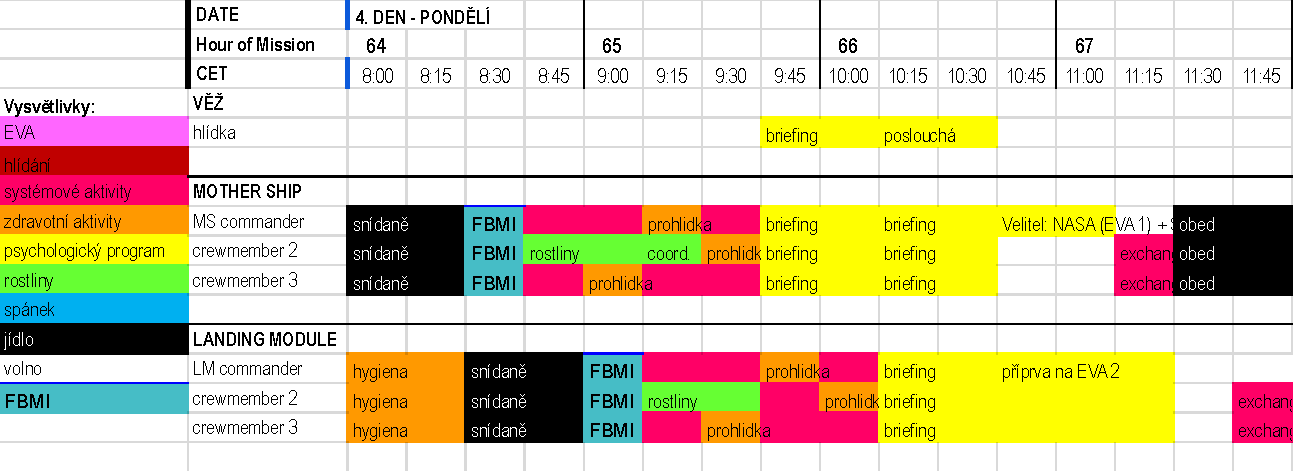
\includegraphics[width=1\linewidth]{figures/harmonogram}
        \end{framed}
        \caption{Ukázka části harmonogramu mise}
        \label{fig:harmonogram}
    \end{center}
\end{figure}

Spolu s harmonogramem byly záznamy všech významných událostí a plán směn. Plán
směn byl vytvořen interně pro každou instituci, jež byla součástí mise. Každá
směna sloužila primárně za účelem monitorování a dokumentace mise.

\subsubsection{Řídicí věž}
\label{subsubsec:ridici_vez}
Řídicí věž hrála v rámci mise DIANA roli stanoviště na Zemi. Komunikovala tedy
se základnou (mateřskou lodí) v souvislosti s prováděním výzkumných a
vzdělávacích programů. Zároveň zde bylo umístěno monitorovací zařízení posádky,
které nepřetržitě sbíralo data a dokumentační a komunikační zařízení.

\begin{figure}[h]
    \begin{center}
        \includegraphics[width=1\linewidth]{figures/monitoring}
        \caption{Monitorování posádky v řídící věži během mise (zdroj: Hydronaut Project a.s.)}
        \label{fig:monitoring}
    \end{center}
\end{figure}

\subsubsection{Povrchová jednotka}
\label{subsubsec:povrchova_jednotka}
Povrchová jednotka byla složena z vedoucího týmu (tři členové stejně jako v
podvodním habitatu), který řídil polohu stanice a systémy podpory života.
Zároveň se povrchová jednotka starala o regulaci specifických parametrů v
závislosti na průběhu mise. Během mise DIANA hrála tato jednotka roli mateřské
lodi, jež sloužila jako stanoviště a kritické zázemí pro velitele posádky. Z
tohoto místa probíhalo ovládání stanice H03 DeepLab.

\subsection{Neuropsychofyziologická baterie}
\label{subsubsec:neuro_testy}
Neuropsychofyziologická stimulace a diagnostika jedinců byla během mise
realizována prostřednictvím následujících nástrojů:
\begin{enumerate}
    \item \textbf{Kognitivní úlohy v prostředí NEUROP-III} --- posádka opakovaně
          podstoupila náročné diagnostické kognitivní úlohy, zvláště zaměřené na
          sledování exekutivních funkcí primárně v oblasti impulzivního chování,
          riskování, interference nebo inhibice ve smyslu Go/No-go.
    \item \textbf{Subjektivní hodnocení pomocí NASA TLX} --- jedná se o
          dlouholetý standard pro měření subjektivního vnímání mentální zátěže
          vzhledem ke konkrétním úkolům v pěti dimenzích: mentální náročnost, fyzická
          náročnost, časová náročnost, výkonnost, snaha a frustrace. Posádka byla
          tímto hodnocena během celé mise každý den.
\end{enumerate}

\subsection{Monitorování a měření posádky}
\label{subsec:monitorovani posadky}
Během celého průběhu mise byla posádka neustále monitorována kamerovým systémem
a měřena pomocí validovaných biometrických zařízení, které poskytovaly palubnímu
počítači údaje o stavu posádky: tepová frekvence, dechová frekvence a kožní
vodivost. Zároveň byly pomocí kamerových záznamů detekovány emoce posádky z
výrazů tváře. Na Obr.~\ref{fig:monitoring} lze vidět snímky z monitorování
posádky během mise DIANA.

\begin{figure}[h]
    \begin{subfigure}[h]{0.48\linewidth}
        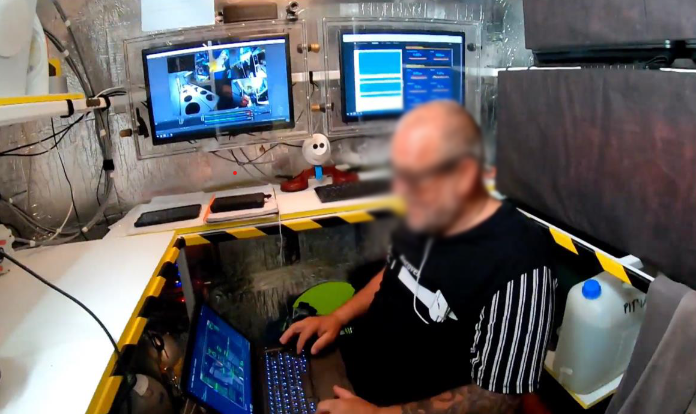
\includegraphics[width=\linewidth]{figures/lander}
        \caption{Snímek z monitorování v přistávacím modulu (interiér modulu)}
    \end{subfigure}
    \hfill
    \begin{subfigure}[h]{0.48\linewidth}
        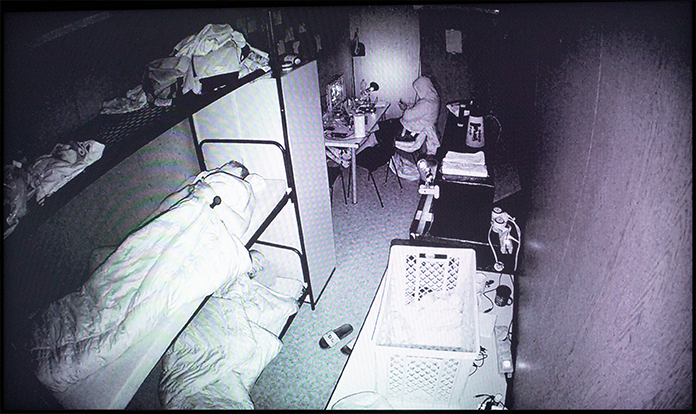
\includegraphics[width=\linewidth]{figures/nightcam}
        \caption{Noční snímek z monitorování posádky mateřské lodi}
    \end{subfigure}
    \caption{Snímky z monitorování posádky během mise (zdroj: Hydronaut Project a.s.)}
\end{figure}

Data z biometrických jednotek byla pomocí bezdrátové sítě WLAN (Wi-Fi 2,4 GHz)
přenášena na datový server a ukládána do InfluxDB. Ostatní kompartmenty mise tak
mohly živě sledovat fyziologický stav posádky. Díky real-time vizualizaci bylo
také možné dohlížet na správností měření biologických signálů. Předcházelo se
tak situacím jako: nesprávně nalepené či odlepené elektrody, přítomnost
elektromagnetického rušení ovlivňujícího měření nebo výpadky způsobené problémy
s bezdrátovým připojením.

\subsubsection{InfluxDB}
\label{subsec:influx}
InfluxDB\footnote{https://www.influxdata.com} je open-source platforma
poskytující databázi pro časové řady. Zahrnuje databázové rozhraní (API).
Součástí je i grafické uživatelské rozhraní (GUI) s modulárními uživatelskými
panely pro monitorování dat v reálném čase. Platforma (InfluxDB OSS 2.4) byla
využita v rámci mise k uchovávání a vizualizaci dat.

\subsubsection{Měření biosignálů}
\label{subsubsec:mereni_biosignalu}
V minulé sekci byla zmínka o biometrických datech jako například tepová a
dechová frekvence. Tato data byla získána pomocí biometrických jednotek, které
však neměří přímo tyto fyziologické indikátory ale biologické signály. Měřenými
biosignály jsou: srdeční, respirační a elektrodermální aktivita. Biosignály byly
zaznamenávaný u šesti jedinců, konkrétně u posádky mateřské lodi a přistávacího
modulu. V následující sekci je detailněji rozebráno měřící zařízení.

\begin{figure}[!htb]
    \begin{center}
        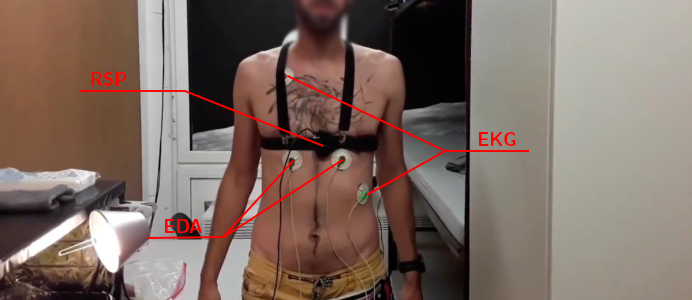
\includegraphics[width=1\linewidth]{figures/sensors}
        \caption{Ukázka měřících čidel na těle člena posádky uvnitř mateřské lodi}
        \label{fig:sensors}
    \end{center}
\end{figure}

\subsubsection{Měřící zařízení}
\label{subsubsec:merici_zarizeni}
Pro měření biosignálu během simulované vesmírné mise byly použity validované
telemedicínské jednotky BoRec (Body Recorder), které jsou dlouhodobě vyvíjené ve
výzkumné skupině Biomechaniky a asistivních technologií na Fakultě
biomedicínského inženýrství (\gls{FBMI}), ČVUT v Praze. Vzorkovací frekvence
zařízení je 250~Hz. Zařízení je možné vidět vidět na Obr.~\ref{fig:borec}.

\begin{figure}[!htb]
    \begin{center}
        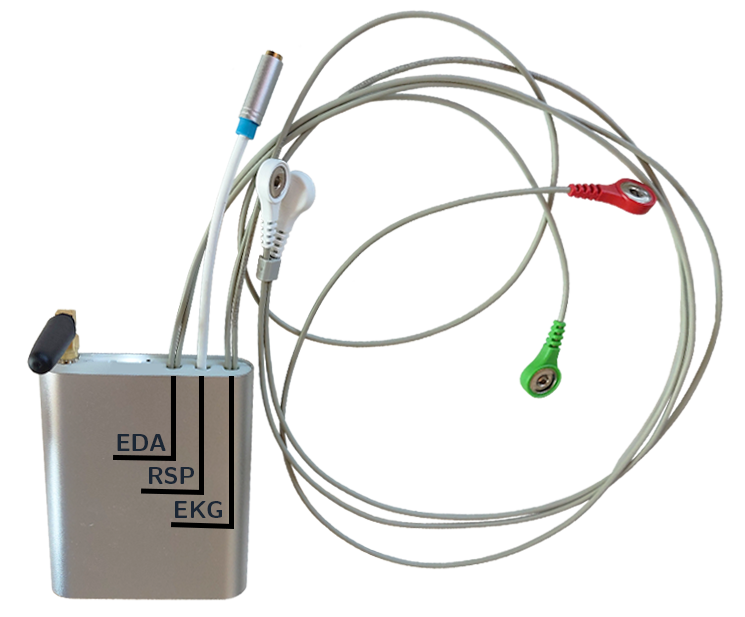
\includegraphics[width=0.6\linewidth]{figures/borec}
        \caption{Telemedicínská jednotka BoRec použita během mise}
        \label{fig:borec}
    \end{center}
\end{figure}

Respirační aktivita byla měřena pomocí dechového pásu, který je založen na
tenzometrickém principu. Elektrodermální aktivita byla měřena pomocí dvou
elektrod na hrudi. Toto místo bylo pro potřeby mise vybráno na základě
studie~\cite{Janssen2012}. Elektrická srdeční aktivita byla měřena využitím
jednosvodového systému, přičemž byl svod zaznamenáván v konfiguraci II. Jednotka
včetně snímačů biosignálů také obsahuje tlakové a gyroakcelometrické senzory.

Bezdrátové připojení jednotek je zajištěno využitím bezdrátové sítě WLAN.
Komunikačním protokol mezi zařízením a klientem na straně počítače je Modbus
TCP~\cite{modbus}, který umožňuje přístup k senzorům jednotky a stažení dat z
vyrovnávacích pamětí. Každá jednotka má svou vlastní jedinečnou MAC adresu a
očekává adresu IP od serveru DHCP. Klient na PC má přístup ke všem snímačům
sítě.

\subsection{Studie}
\label{subsec:studie}
Měření dat probíhalo v rámci projektu pod Filozofickou fakultou Univerzity
Palackého v Olomouci (\gls{FF UPOL}). Všichni probandi poskytli informované
souhlasy pro část diagnostickou i pro samotný experiment (viz
Příloha~\ref{appendix:a}). Informované souhlasy umožňují anonymizované využití
dat. Získání dat pod FF UPOL probíhalo podle etického metakodexu Evropské
federace psychologických asociací (\gls{EFPA}). Informované souhlasy jsou i ke
všem nahrávkám obrazových dat a rozhovorů členů posádky. Bezpečí participantů
bylo jištěno v několika technických rovinách prostřednictvím hlavního řešitele
\textit{1st Cloud Republic a.s.} projektu TL05000228.